\documentclass[11pt]{article}

\usepackage[spanish]{babel}
\usepackage[margin=1in]{geometry}
\usepackage{amsmath, amssymb, amsfonts}
\usepackage{graphicx}
\usepackage{float}
\usepackage{booktabs}
\usepackage{enumitem}
\usepackage{tcolorbox}
\usepackage{hyperref}
\usepackage{listings}
\usepackage{xcolor}
\usepackage{parskip}
\usepackage{pgfplots}

\usetikzlibrary{arrows.meta}
\pgfplotsset{compat=1.18}

\lstset{
  language=Python,
  basicstyle=\ttfamily\footnotesize,
  breaklines=true,
  columns=flexible,
  keepspaces=true,
  commentstyle=\color{gray}\itshape,
  keywordstyle=\color{blue!70!black}\bfseries,
  stringstyle=\color{green!40!black},
  frame=L,
  xleftmargin=2em,
  showstringspaces=false,
  tabsize=4
}

\lstset{language={}, basicstyle=\ttfamily\footnotesize, inputencoding=utf8, extendedchars=true,
  literate={á}{{\'a}}1 {é}{{\'e}}1 {í}{{\'i}}1 {ó}{{\'o}}1 {ú}{{\'u}}1 {ñ}{{\~n}}1
           {Á}{{\'A}}1 {É}{{\'E}}1 {Í}{{\'I}}1 {Ó}{{\'O}}1 {Ú}{{\'U}}1 {Ñ}{{\~N}}1 {≈}{{$\approx$}}1}
\setlist{itemsep=2pt, topsep=4pt}

\title{\textbf{Laboratorio 8: Mini-GPT, estrategias de muestreo y embeddings contextuales} \vspace{1em}\\
  Deep Learning y Sistemas Inteligentes - CC3092}
\author{José Antonio Mérida Castejón}
\date{\today}

\begin{document}
\decimalpoint

\maketitle

\section*{Nota sobre este documento}
Este documento recopila las respuestas de cada task. Todo el trabajo (código, salidas, gráficas y respuestas) ya se realizó en el notebook \texttt{Notebook.ipynb}, entregado junto con este PDF; aquí se reproducen las mismas respuestas y resultados. Las muestras generadas completas están en el apéndice~\ref{app:samples}.

\section*{Task 1}

\subsection*{Task 1.1 --- Dataset, vocabulario y batches}
Se descargó \texttt{tiny\_shakespeare} (1,115,394 caracteres). El vocabulario tiene exactamente 65 caracteres, y la partición 90/10 respeta el orden temporal: 1,003,854 caracteres de entrenamiento y 111,540 de validación. Los batches tienen forma $(64, 128)$ y la secuencia objetivo es la de entrada desplazada un paso (comprobado en el notebook). Hiperparámetros: \texttt{block\_size} = 128, \texttt{d\_model} = 128, \texttt{n\_heads} = 4, \texttt{n\_layers} = 3, \texttt{batch\_size} = 64, \texttt{lr} = 3e-4.

\subsection*{Mini-GPT}
Se reutiliza la implementación del \texttt{MiniGPT} de la Semana 6 (\texttt{S6\ -\ Proyecto1\_Semana6.ipynb}) con \textbf{los mismos bloques}. Utiliza parámetros crudos \texttt{nn.Parameter} (sin \texttt{nn.MultiheadAttention} ni capas de alto nivel), \texttt{layer\_norm} propio, positional encoding sinusoidal de Vaswani et al., atención multi-cabeza con máscara causal (\texttt{-inf} en el triángulo superior antes del softmax), FFN con ReLU y esquema \emph{Post-LN} (Add \& LayerNorm).

\textbf{Cambios necesarios respecto a la Semana 6} (por lo que pide este laboratorio):

\begin{itemize}
\item
  Vocabulario de \textbf{caracteres} (65) en lugar de palabras de SST-2; no hay tokens \texttt{\textless{}PAD\textgreater{}/\textless{}BOS\textgreater{}/\textless{}EOS\textgreater{}}.
\item
  Procesamiento por \textbf{batches} \texttt{(B,\ T)} en vez de una oración a la vez \texttt{(T,)}.
\item
  \textbf{\texttt{n\_layers\ =\ 3}} bloques apilados (antes 1) y \texttt{d\_model=128}, \texttt{n\_heads=4} (antes 32 y 2). \texttt{d\_k\ =\ d\_model\ /\ n\_heads\ =\ 32}.
\item
  \texttt{d\_ff\ =\ 4\ *\ d\_model} (en la Semana 6 era \texttt{2\ *\ d\_model}).
\item
  La inicialización \texttt{N(0,\ 0.1)} se mantiene igual que en la Semana 6.
\end{itemize}

El modelo tiene 609,985 parámetros. La verificación de causalidad del notebook confirma que cambiar un token futuro no altera las posiciones anteriores.

\subsection*{Task 1.2 --- Entrenamiento, curvas y perplejidad de validación}
\textbf{Nota sobre \texttt{epochs}:} el enunciado lista \texttt{epochs\ =\ 10} entre los hiperparámetros \emph{mínimos}. Con 10 épocas reales ($\approx$1,230 pasos) el modelo queda subentrenado (la perplejidad de validación es $\approx$8.24), fuera del rango esperado {[}3.5, 8.0{]} y la pérdida seguía bajando. Como se trata de valores mínimos, se entrena durante \textbf{35 épocas} ($\approx$4,300 pasos); el resto de hiperparámetros no cambia. Se usa además un \emph{warmup} lineal del learning rate (lr máximo = 3e-4).

\begin{table}[H]
\centering
\begin{tabular}{lrrr}
\toprule
Época & Pérdida de entrenamiento & Pérdida de validación & Perplejidad de validación \\
\midrule
10 & 2.0786 & 2.1094 & 8.244 \\
35 & 1.5732 & 1.7654 & 5.844 \\
\bottomrule
\end{tabular}
\end{table}

\begin{figure}[H]
\centering
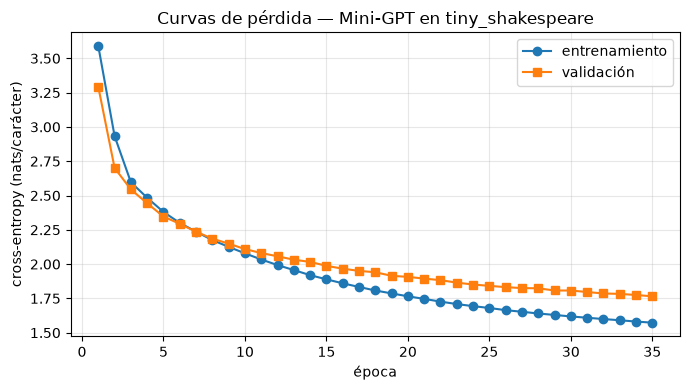
\includegraphics[width=0.75\textwidth]{figs/curvas_perdida.png}
\end{figure}

Perplejidad de validación $=\exp(1.7654)=5.844$, dentro del rango esperado $[3.5, 8.0]$.

Queda confirmado que con los hiperparámetros elegidos la perplejidad se encuentra dentro del rango de validación y la curva de pérdida muestra que el modelo convergió. Basado en la curva, empezó a overfittear ligeramente pero probablemente dejarlo algunas épocas más con algun decay de LR dé mejores resultados.

\subsection*{Task 1.3 --- Funciones de muestreo}
Las tres funciones (greedy, top-k con temperatura y top-p con temperatura) están implementadas desde cero en el notebook, reciben los logits crudos y retornan el índice del siguiente token.

\section*{Task 2}

\subsection*{Task 2.1 --- \texttt{generate()} y muestras}
Se generaron 5 muestras de 200 caracteres por configuración, partiendo de \texttt{ROMEO:}.
\begin{table}[H]
\centering
\begin{tabular}{lll}
\toprule
Configuración & Estrategia & Parámetros \\
\midrule
A & greedy & ninguno \\
B & top-k & $k=5$, $\tau=0.7$ \\
C & top-k & $k=50$, $\tau=1.0$ \\
D & top-p & $p=0.70$, $\tau=0.7$ \\
E & top-p & $p=0.95$, $\tau=1.0$ \\
\bottomrule
\end{tabular}
\end{table}

\subsection*{Task 2.2 --- Análisis de las muestras}

\subsubsection*{(a) ¿Por qué greedy (config. A) repite o entra en ciclos?}
Greedy elige \(w_{t+1}=\arg\max_i z_i\). Es decir, es una función determinista que dado el mismo contexto siempre produce el mismo carácter y descarta completamente el resto. El comportamiento repetitivo se puede observar en las 5 muestras idénticas (al ser determinista) que caen en un ciclo de repeticiones de ``the stay'', ``the see'', ``the stand''.

\begin{lstlisting}
Why, there the stay the see the stay the stand
That the stay the stay the stand the stay the seem
Than the stay the seem the seem the seem and the seembers
The can the seems and the seember the seemb
\end{lstlisting}

Esto ocurre porque, aunque en muchas posiciones la distribución del siguiente carácter está repartida entre varias opciones plausibles, greedy descarta toda esa masa y se queda siempre con la opción más probable dado el contexto. Esta suele ser una continuación muy común, por ejemplo, palabras funcionales como \texttt{the}. Al ser determinista, basta con que el contexto llegue a un estado donde el \texttt{argmax} lleve de vuelta a una secuencia ya vista para que el texto caiga en un ciclo.

\subsubsection*{(b) Config. B (top-k, $k=5$, $\tau=0.7$) vs. C (top-k, $k=50$, $\tau=1.0$)}
Con temperatura, la probabilidad de cada carácter es

\[P(w_i \mid ctx) = \frac{\exp(z_i/\tau)}{\sum_j \exp(z_j/\tau)}\]

En top-k, la suma del denominador solo incluye los \(k\) caracteres con mayor logit. El resto tiene probabilidad 0.

El parámetro \(k\) fija cuántos caracteres pueden muestrearse en cada paso. Con \(k=5\) el modelo solo elige entre los cinco más probables, así que casi todo lo que genera son palabras reales y frecuentes. Por ejemplo, B1 produce ``The death shall now and to my thank he streate, And the come a see of the cale have at strange.'' A cambio, el texto repite mucho las palabras funcionales, como ``be be'' en B5, ``to thee come with thee world'' en B2 o ``the wear the will'' en B1. Con \(k=50\) casi no hay recorte, ya que el vocabulario tiene 65 caracteres. Entran caracteres poco probables y el texto se vuelve más variado pero también más ruidoso. Aparecen palabras inventadas como ``withipinus'' y ``nisur'' en C1 o ``seepinated's'' y ``petteignness'' en C5, y también más signos de puntuación.

La temperatura divide los logits antes del softmax, así que cambia qué tan separadas quedan las probabilidades. Si dos caracteres tienen logits que difieren en 1, el ratio entre sus probabilidades es \(e^{1/\tau}\). Con \(\tau=1.0\) ese ratio es \(e^{1} \approx 2.7\), y con \(\tau=0.7\) es \(e^{1/0.7} \approx 4.2\). Es decir, con \(\tau=0.7\) el carácter más probable gana todavía más peso frente a los demás y la distribución se concentra. Con \(\tau=1.0\) se usa la distribución original del modelo, que es más plana y le da más peso a las opciones poco probables.

Hay una limitación importante. B y C cambian ambos parámetros a la vez, así que estas muestras no permiten aislar el efecto de \(k\) y el de \(\tau\) por separado. Lo que se observa es consistente con lo que predice la fórmula, pero no lo prueba por sí solo.

En cuanto a coherencia y creatividad, B es la más coherente a nivel de palabras, porque casi todas existen en inglés. Esto tiene sentido porque los cinco caracteres más probables suelen ser continuaciones razonables, mientras que el carácter número 30 o 50 casi nunca lo es. En C cada uno de esos caracteres tiene probabilidad baja, pero juntos suman una masa que no es despreciable, sobre todo con \(\tau=1.0\). A lo largo de 200 caracteres es casi seguro que en algún momento se elija uno de ellos, y basta un solo carácter malo para romper una palabra. Además, ese error queda en el contexto y afecta las predicciones siguientes. Por eso C es la más diversa y creativa, pero produce muchas pseudo-palabras. B en cambio, no forma frases con sentido y es repetitiva, porque siempre se mueve entre las mismas opciones seguras.

\subsubsection*{(c) Config. E (top-p $=0.95$, $\tau=1.0$): momentos de seguridad e incertidumbre}
El tamaño del núcleo depende de la forma de la distribución en cada paso. Si el modelo está seguro, un solo carácter puede acumular casi toda la probabilidad y el núcleo es muy pequeño. Si está inseguro, la probabilidad está repartida y hacen falta muchos caracteres para llegar a 0.95.

Para respaldar esto con datos, la celda anterior genera una muestra adicional con la configuración E y registra en cada paso la probabilidad máxima \(p_{\max}\) y el tamaño del núcleo. Los números se refieren a esa muestra y no a E1 a E5, pero el mismo comportamiento se ve en las cinco muestras.

El modelo está muy seguro en posiciones de puntuación, formato y continuaciones obvias de palabra. En todos estos casos el núcleo tiene un solo carácter. Después de los dos puntos que cierran el nombre de un personaje, el siguiente carácter es un salto de línea con \(p_{\max}=0.99\). Esto se ve en todas las muestras, donde nombres como ``RARCHIS:'', ``MARDIUS:'' o ``KING RICHARD II:'' siempre van seguidos de un salto de línea. Algo parecido pasa después de un punto, donde viene un salto de línea con \(p_{\max}=0.98\), y después de una coma o al final de una palabra, donde viene un espacio con \(p_{\max}\) entre 0.95 y 0.96. También hay continuaciones casi forzadas dentro de las palabras. Después de una ``i'' el modelo elige ``n'' con \(p_{\max}=0.95\), y después de una ``n'' elige ``g'' con \(p_{\max}=0.97\). Esto es consistente con la terminación ``-ing'', que es muy frecuente en el corpus y que el modelo incluso aplica a palabras inventadas como ``Thereing'' o ``childing''. En todos estos casos el corpus es casi determinista, así que la distribución se concentra en una sola opción.

El modelo está inseguro en las fronteras de palabra y de línea. Los casos más inciertos son casi todos la primera letra de una palabra, justo después de un espacio. Ahí el núcleo tiene entre 24 y 30 de 65 caracteres y \(p_{\max}\) está entre 0.12 y 0.23, porque elegir qué palabra viene es una decisión muy abierta. Al empezar una línea nueva pasa algo parecido, con un núcleo de 24 caracteres y \(p_{\max}\) entre 0.21 y 0.31. El modelo no sabe qué personaje o qué palabra abre la línea, y es justo ahí donde aparecen los nombres inventados de las muestras, como ``RARCHIS'' o ``KICHARD ING HERMARD III''. Una vez que la palabra empezó, las opciones se reducen y la incertidumbre baja.

En total, el núcleo tuvo en promedio unos 9.1 caracteres, con valores entre 1 y 30. Esto muestra la adaptatividad que describe el enunciado. Un top-k fijo usaría siempre el mismo número de candidatos, mientras que top-p usa uno solo cuando el modelo está seguro y hasta 30 cuando no lo está.

\section*{Task 3}

\subsection*{Task 3.1 --- Embeddings contextuales de \texttt{bert-base-multilingual-cased}}
\subsection{\texorpdfstring{Task 3.1 --- Embeddings contextuales de \texttt{bert-base-multilingual-cased}}{Task 3.1 --- Embeddings contextuales de bert-base-multilingual-cased}}\label{task-3.1-embeddings-contextuales-de-bert-base-multilingual-cased}

Para cada oración se toma el estado oculto de la \textbf{última capa} (\texttt{last\_hidden\_state}, dimensión 768) en la posición de la palabra objetivo (no \texttt{{[}CLS{]}}). Si WordPiece parte la palabra en varios sub-tokens, se promedian sus vectores; si es un solo token, es directamente ese vector. La posición se localiza con \texttt{offset\_mapping} (caracteres de la palabra en la oración), no buscando el texto del token, para no confundirla con otras apariciones.

En las 7 oraciones la palabra objetivo es un único sub-token y cada embedding tiene dimensión 768.

\subsection*{Task 3.2 --- Similitud coseno, Word2Vec y PCA}

\subsubsection*{(a) Similitud coseno entre contextos distintos de la misma palabra (BERT)}
\[
\text{sim}(\mathbf{u},\mathbf{v}) = \frac{\mathbf{u}^\top \mathbf{v}}{\lVert\mathbf{u}\rVert\,\lVert\mathbf{v}\rVert}
\]
\begin{table}[H]
\centering
\begin{tabular}{llll}
\toprule
Palabra & Contexto 1 & Contexto 2 & Coseno BERT \\
\midrule
banco & institución financiera & asiento & 0.5753 \\
banco & institución financiera & cardumen & 0.6603 \\
banco & asiento & cardumen & 0.6496 \\
copa & trofeo & recipiente & 0.5667 \\
vela & de barco & cirio & 0.7999 \\
\bottomrule
\end{tabular}
\end{table}

\subsubsection*{(b) Vectores estáticos Word2Vec y comparación con BERT}
El descargador de gensim no incluye modelos en español, así que se carga desde el Hub de HuggingFace \texttt{Word2vec/wikipedia2vec\_eswiki\_20180420\_300d} (vectores de 300 dimensiones tipo skip-gram entrenados sobre Wikipedia en español, formato Word2Vec de texto) con \texttt{gensim.models.KeyedVectors}. Un modelo estático asigna \textbf{un único vector por palabra}, sin importar la oración, por lo que la similitud entre dos contextos de la misma palabra es 1.0 por construcción. Esto no es un hallazgo empírico; es justamente la limitación que BERT corrige.

\begin{table}[H]
\centering
\begin{tabular}{llllrr}
\toprule
Palabra & Contexto 1 & Contexto 2 & Coseno BERT & Coseno Word2Vec & BERT $-$ Word2Vec \\
\midrule
banco & institución financiera & asiento & 0.5753 & 1.0 & $-0.4247$ \\
banco & institución financiera & cardumen & 0.6603 & 1.0 & $-0.3397$ \\
banco & asiento & cardumen & 0.6496 & 1.0 & $-0.3504$ \\
copa & trofeo & recipiente & 0.5667 & 1.0 & $-0.4333$ \\
vela & de barco & cirio & 0.7999 & 1.0 & $-0.2001$ \\
\bottomrule
\end{tabular}
\end{table}

Vecinos más cercanos en Word2Vec: \texttt{banco}: hipotecario, sudameris, bancos, totalbank, finantia, banex; \texttt{copa}: supercopa, recopa, copas, redireccióncopa, libertadores, cup; \texttt{vela}: enverga, envergada, rfev, envergar, gennaker, contromano.

Con Word2Vec la similitud es 1.0 en todos los pares, esto es una consecuencia de cómo funciona el modelo. Word2Vec es estático y guarda un solo vector por palabra, así que ``banco'' tiene el mismo vector sin importar la oración en la que aparece. No puede distinguir entre diferentes sentidos semánticos.

Los vecinos más cercanos muestran qué sentido domina ese vector. Para ``banco'' son ``hipotecario'', ``bancos'' o ``banex'', todos del sentido financiero. Para ``copa'' son ``supercopa'', ``recopa'' o ``libertadores'', del sentido de trofeo. Para ``vela'' son términos de navegación como ``enverga'', ``envergada'' o ``gennaker''. Como el vector se aprende de todas las apariciones de la palabra en Wikipedia, queda dominado por el sentido más frecuente. Los sentidos menos comunes, como banco de asiento o vela de cirio, casi no se reflejan.

BERT, en cambio, sí separa los sentidos. Sus similitudes van de 0.57 a 0.80, claramente por debajo de 1, porque cada vector depende de la oración completa. El par con mayor similitud es el de ``vela'' con 0.80, lo que sugiere que BERT separó menos esos dos sentidos. Aun así, como hay una sola oración por sentido las diferencias pequeñas entre pares pueden deberse a las oraciones específicas y no tanto al sentido. Se deberían de analizar más oraciones utilizando cada una de las palabras en sus diferentes sentidos.

\subsubsection*{(c) Visualización con PCA (2D) de los embeddings de BERT}
Cada punto es una instancia de la palabra en su contexto (7 en total). El color indica el significado y la forma indica la palabra. El PCA se ajusta sobre las 7 instancias juntas (varianza explicada: PC1 35\%, PC2 23.5\%).

\begin{figure}[H]
\centering
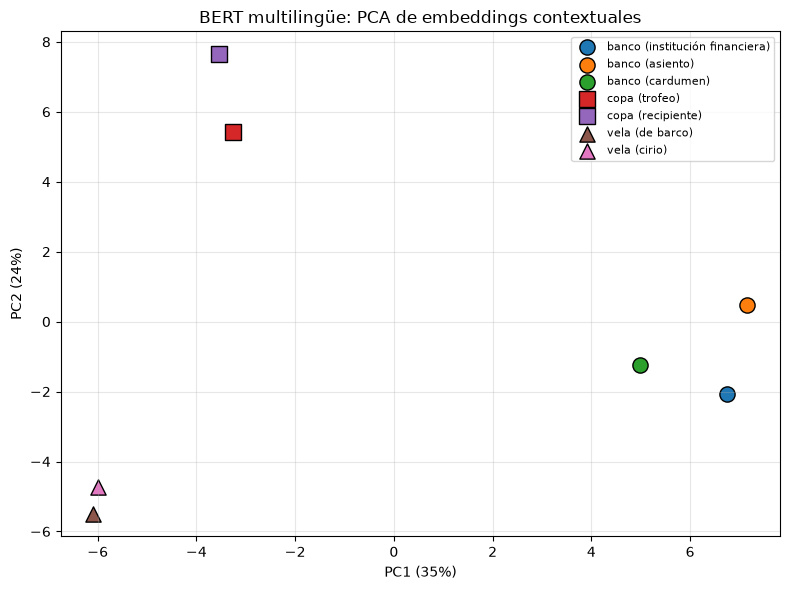
\includegraphics[width=0.75\textwidth]{figs/pca_bert.png}
\end{figure}

En la proyección PCA los puntos se agrupan por palabra y no por significado. Se forman tres grupos claros:

\begin{itemize}
\item
  Los tres ``banco'' a la derecha
\item
  Los dos ``copa'' arriba a la izquierda
\item
  Los dos ``vela'' abajo a la izquierda.
\end{itemize}

Dentro de cada grupo los distintos sentidos aparecen como puntos separados, así que BERT sí les asigna vectores diferentes. Sin embargo, la distancia entre sentidos de una misma palabra es mucho menor que la distancia entre palabras distintas. Es decir, la mayor fuente de variación en el espacio es qué palabra es, y el contexto solo la desplaza un poco dentro de su grupo.

Esto es consistente con las similitudes coseno de la tabla anterior. Los dos sentidos de ``vela'' quedan casi encima uno del otro, lo que coincide con su similitud de 0.80. En ``banco'', el sentido de asiento queda algo apartado de los otros dos y es justo el par con menor similitud frente al sentido financiero. La visualización en dos dimensiones puede no ser la comparación más precisa, pero si podemos concluir que los contextos distintos sí se separan, pero dentro del espacio de la palabra y no como grupos independientes por significado.

\section*{Task 4}

\subsection*{Task 4.1 --- Preguntas conceptuales}

\subsubsection*{(a) Máscara causal y atención bidireccional}
El objetivo de language modeling factoriza la probabilidad de una secuencia como

\[P(x_1,\dots,x_T)=\prod_t P(x_t\mid x_{<t})\]

Para que el modelo estime \(P(x_t\mid x_{<t})\), la representación en la posición \(t\) solo puede depender de los tokens anteriores. La máscara causal logra esto sumando \(-\infty\) a los scores de atención con \(j>i\) antes del softmax, así que esos pesos quedan exactamente en 0. Esto es necesario porque en el entrenamiento todas las posiciones se calculan en paralelo con teacher forcing. Sin la máscara, la posición \(t\) podría ver el token \(x_{t+1}\), que es su etiqueta.

Si GPT usara atención bidireccional en el preentrenamiento, predecir el siguiente token se volvería trivial. El modelo aprendería a copiar \(x_{t+1}\) desde la entrada y la pérdida caería casi a 0 sin que aprendiera mucho sobre el lenguaje. Además, el modelo ya no definiría una distribución \(P(x_t\mid x_{<t})\) válida. El problema aparece en la generación, porque ahí el siguiente token todavía no existe. Lo que el modelo aprendió a hacer ya no sirve y hay una discrepancia entre cómo se entrenó y cómo se usa.

\subsubsection*{(b) Preentrenar y adaptar: GPT vs. BERT}
En el Task 3, BERT dio vectores distintos para la misma palabra en contextos distintos con similitudes coseno entre 0.57 y 0.80, mientras que Word2Vec dio 1.0 en todos los casos. Esto pasa porque BERT calcula cada token atendiendo a la oración completa, tanto a la izquierda como a la derecha. Esa propiedad es útil para tareas de comprensión, como clasificación, desambiguación, similitud o extracción de entidades. GPT con atención causal, solo ha visto el contexto anterior cuando llega a ``banco''. Su representación en ese punto no puede usar lo que viene después como ``del parque'' o ``de peces'', que es justo lo que define el sentido. A cambio, GPT sí define \(P(x_t\mid x_{<t})\) y puede generar texto, como hicimos en el Task 2.

El paradigma de preentrenar y adaptar resuelve esta tensión porque ambos modelos ya fueron preentrenados con grandes corpus. No hace falta entrenar ninguno desde cero, solo elegir el adecuado para la tarea. Si la tarea es entender o clasificar texto, se usa BERT y se le agrega una capa pequeña o se hace fine-tuning, partiendo de embeddings como los del Task 3. Si la tarea es generar o continuar texto, se usa GPT con prompting o fine-tuning. El costo grande de aprender el lenguaje se paga una sola vez en el preentrenamiento, y la adaptación a cada tarea es barata.

Nuestros resultados también muestran por qué la adaptación importa. La separación de significados en BERT fue parcial. Los dos sentidos de ``vela'' tuvieron una similitud de 0.80, y en el PCA los puntos se agruparon por palabra y no por significado. Por eso, para una desambiguación fina conviene hacer fine-tuning en lugar de usar los embeddings congelados tal cual.

\newpage
\appendix
\section{Muestras generadas (Task 2.1)}\label{app:samples}
\subsection*{Configuración A: \{'strategy': 'greedy'\}}
\textbf{Muestra A1}
\begin{lstlisting}
ROMEO:
Why, there the stay the see the stay the stand
That the stay the stay the stand the stay the seem
Than the stay the seem the seem the seem and the seembers
The can the seems and the seember the seemb
\end{lstlisting}
\textbf{Muestra A2}
\begin{lstlisting}
ROMEO:
Why, there the stay the see the stay the stand
That the stay the stay the stand the stay the seem
Than the stay the seem the seem the seem and the seembers
The can the seems and the seember the seemb
\end{lstlisting}
\textbf{Muestra A3}
\begin{lstlisting}
ROMEO:
Why, there the stay the see the stay the stand
That the stay the stay the stand the stay the seem
Than the stay the seem the seem the seem and the seembers
The can the seems and the seember the seemb
\end{lstlisting}
\textbf{Muestra A4}
\begin{lstlisting}
ROMEO:
Why, there the stay the see the stay the stand
That the stay the stay the stand the stay the seem
Than the stay the seem the seem the seem and the seembers
The can the seems and the seember the seemb
\end{lstlisting}
\textbf{Muestra A5}
\begin{lstlisting}
ROMEO:
Why, there the stay the see the stay the stand
That the stay the stay the stand the stay the seem
Than the stay the seem the seem the seem and the seembers
The can the seems and the seember the seemb
\end{lstlisting}
\subsection*{Configuración B: \{'strategy': 'top-k', 'k': 5, 'tau': 0.7\}}
\textbf{Muestra B1}
\begin{lstlisting}
ROMEO:
The death shall now and to my thank he streate,
And the come a see of the cale have at strange.
What it is the comfort than to they stand are saw the change
By to be shall the wear the will burined a
\end{lstlisting}
\textbf{Muestra B2}
\begin{lstlisting}
ROMEO:
I was thou be the come honour to thee come with thee world
That their we hearts the duke a counteds to thee strain,
Thou what we sin the doth of hearts him here heart;
That what tendering a the broth
\end{lstlisting}
\textbf{Muestra B3}
\begin{lstlisting}
ROMEO:
And the despered to most streaks an on my father,
And think the parts of all the shall bear preate
This news as may the death, then to me sistelf the was,
And this set strand they to him the stranges
\end{lstlisting}
\textbf{Muestra B4}
\begin{lstlisting}
ROMEO:
I say the sure shall be the dear that the consurs
To stay thou hereads and me for hunder than are the but a so may
The dispering the changer of the doth on the words.

LUCIO:
Trutter it my lords to t
\end{lstlisting}
\textbf{Muestra B5}
\begin{lstlisting}
ROMEO:
Why, thy will I spay at my lieges on his hander the cound of my lords.

CAMILLO:
So, my leaves the king's hearts the was that
That shall be be thanks in that stone mon,
And I win am that sending this
\end{lstlisting}
\subsection*{Configuración C: \{'strategy': 'top-k', 'k': 50, 'tau': 1.0\}}
\textbf{Muestra C1}
\begin{lstlisting}
ROMEO:
Honry mise, now cure heart; the this out stubh
Inle to grace's sorrow in them wine put dendam,
My withipinus Caul show he: and nisur,
Would read's his beand, and she bear'd of my ear both,
Were any V
\end{lstlisting}
\textbf{Muestra C2}
\begin{lstlisting}
ROMEO:
My lange be thine!

DUkis Mancasted curl-binatouraty a sear.

Promer:
We honous am with:
And lorneis, tee-joy!

POLIXENES:
How 'It your them beeects where a not whom prace hands!
For most be honours!
\end{lstlisting}
\textbf{Muestra C3}
\begin{lstlisting}
ROMEO:
As I would compare form siting seedf,
With child the conful death. Then and befores,
Mine Duke absued accousin in Senaniss and not for a extray
And the doubtitor, with must sworth mother: All proth,
\end{lstlisting}
\textbf{Muestra C4}
\begin{lstlisting}
ROMEO:
Well, frow's had you curk bother, here cart resolus wish,
The prey let libe bones that me spares'st nure aloney
To prove to that ray-wonguing, get unkeet's Rod!
Lords Horry had think thee our your to
\end{lstlisting}
\textbf{Muestra C5}
\begin{lstlisting}
ROMEO:
Shepher'd pity fould a Strank Angick.

ELBOKE:
God--say honour both slads seepinated's you Frink
Shall the protier'sfort, 'sford, petteignness, freated
Of lone shurptay.

PEOTARES:
I om naw sove done
\end{lstlisting}
\subsection*{Configuración D: \{'strategy': 'top-p', 'p': 0.7, 'tau': 0.7\}}
\textbf{Muestra D1}
\begin{lstlisting}
ROMEO:
I am she heart to the stay for a the bear
With him the king the comest the done.

CAPULET:
The not should the call the with my for made thee.

CLARENCE:
I warwer you thank the will the bear with me b
\end{lstlisting}
\textbf{Muestra D2}
\begin{lstlisting}
ROMEO:
So her come to the can strick and stire to the calling.

DUKE VINCENTIO:
I was not a the consenets and should the so and my love,
And many beat so he can the many of the dukes that the sendeed of the
\end{lstlisting}
\textbf{Muestra D3}
\begin{lstlisting}
ROMEO:
And we will shall thee carrents of the call the bear.

Second MARCIUS:
Ay, I have the come were the man of your will be made my with the bear the we with the sead;
If that not my be storrow thee the
\end{lstlisting}
\textbf{Muestra D4}
\begin{lstlisting}
ROMEO:
The must that the part and stoners his his death
The struther that beging me so see stay.

DUKE OF AUMERLE:
Not it whose have sould his and and with soul his will burth,
What the sender of the can th
\end{lstlisting}
\textbf{Muestra D5}
\begin{lstlisting}
ROMEO:
And we have so me stay the more to speak,
And the with the conter of this confess them be thee,
The come and the been a ware thee a prost and thee,
Thou will the well the persing so my lord,
Then com
\end{lstlisting}
\subsection*{Configuración E: \{'strategy': 'top-p', 'p': 0.95, 'tau': 1.0\}}
\textbf{Muestra E1}
\begin{lstlisting}
ROMEO:
We cleang tell we bound too
withing unal to welling: wome hows,
Too deely my but, till bing sholding with thy news
Matek gone self newsed from now caste thou reartions
Longue of York the father
Warli
\end{lstlisting}
\textbf{Muestra E2}
\begin{lstlisting}
ROMEO:
Itwixt the not, good wis thing; 'thaples,
And people agains?

RARCHIS:
Now, and pity sove be, but, sir desen,
Lory not marks lover. well.

MARDIUS:
I morre your have, dely, bean you, 'tis not:
Were s
\end{lstlisting}
\textbf{Muestra E3}
\begin{lstlisting}
ROMEO:
Naily have your and that lige, I'll my for
Your stantage, and meny; her seet's creates
Agal of this title both cartage'd of doth course my long,
To me worde in not so green is than the knowns never,
\end{lstlisting}
\textbf{Muestra E4}
\begin{lstlisting}
ROMEO:
They langion? In deather hast give
Of letterity; sir, of look thou worth seem's trese it; of she yet yet:
Then shalt never'd in kinged wited? bady thouse a deem.

KICHARD ING HERMARD III:
How word, a
\end{lstlisting}
\textbf{Muestra E5}
\begin{lstlisting}
ROMEO:
If now, straing withal sorration; at with stay's pace.
The shands who struck whing then life.

KING RICHARD II:
We hone hearts they with inst that their pinder,
O, beholer to I'll firy grief; where t
\end{lstlisting}

\section{Estadísticas de la configuración E (apoyo para Task 2.2c)}
\begin{lstlisting}
ROMEO:
Why label came
To childre on childing milder, my lord,
Thereing then leark thy boot of my age:
Nor meeto's neights: gart thee, crave the swet those those.
And this back nothing to thou, much me earth 

Más SEGUROS (menor tamaño de núcleo, mayor prob. máx.):
  contexto ...':' -> '\n'  | p_max=0.99 | núcleo=1
  contexto ...'s' -> 'e'  | p_max=0.99 | núcleo=1
  contexto ...'r' -> 'd'  | p_max=0.98 | núcleo=1
  contexto ...'.' -> '\n'  | p_max=0.98 | núcleo=1
  contexto ...'r' -> 'e'  | p_max=0.97 | núcleo=1
  contexto ...'n' -> 'g'  | p_max=0.97 | núcleo=1
  contexto ...'y' -> ' '  | p_max=0.96 | núcleo=1
  contexto ...'h' -> 't'  | p_max=0.96 | núcleo=1
  contexto ...'s' -> 'e'  | p_max=0.96 | núcleo=1
  contexto ...',' -> ' '  | p_max=0.95 | núcleo=1
  contexto ...'i' -> 'n'  | p_max=0.95 | núcleo=1
  contexto ...'o' -> ' '  | p_max=0.95 | núcleo=1
Más INSEGUROS (mayor tamaño de núcleo, menor prob. máx.):
  contexto ...' ' -> 'm'  | p_max=0.17 | núcleo=30
  contexto ...' ' -> 't'  | p_max=0.17 | núcleo=28
  contexto ...' ' -> 'm'  | p_max=0.14 | núcleo=27
  contexto ...' ' -> 't'  | p_max=0.17 | núcleo=27
  contexto ...' ' -> 'c'  | p_max=0.23 | núcleo=27
  contexto ...' ' -> 'g'  | p_max=0.13 | núcleo=26
  contexto ...' ' -> 't'  | p_max=0.17 | núcleo=26
  contexto ...' ' -> 'c'  | p_max=0.17 | núcleo=25
  contexto ...' ' -> 'c'  | p_max=0.12 | núcleo=24
  contexto ...'\n' -> 'T'  | p_max=0.21 | núcleo=24
  contexto ...' ' -> 't'  | p_max=0.21 | núcleo=24
  contexto ...'\n' -> 'T'  | p_max=0.31 | núcleo=24

Núcleo medio: 9.1 de 65 tokens
\end{lstlisting}

\end{document}
